\documentclass[
	parskip=half,
	a4paper,
]{scrarticle}

\usepackage{xcolor}
\definecolor{seeblau}{HTML}{00A9E0}
\definecolor{seegrau}{HTML}{9AA0A7}

\definecolor{seeblau1}{HTML}{CCEEF9}
\definecolor{seeblau2}{HTML}{A6E1F4}
\definecolor{seeblau3}{HTML}{59C7EB}
\definecolor{seeblau4}{HTML}{00A9E0}
\definecolor{seeblau5}{HTML}{008ECE}


\usepackage{graphicx}
\usepackage{amsmath}
\usepackage{subcaption}
\usepackage{wrapfig}
\usepackage[english]{babel}
\usepackage{blindtext}
\usepackage{microtype}
\usepackage{siunitx}
\usepackage[utf8]{inputenc}
\usepackage{csquotes}
\usepackage{nicefrac}
\usepackage[T1]{fontenc}
\usepackage{amsfonts}
\usepackage{amssymb}
\usepackage{tikz}
\usepackage{parskip}

\usepackage{libertinus, libertinust1math}
\usepackage[sfdefault]{biolinum}
\usepackage{roboto}

\setkomafont{disposition}{\normalfont\sffamily}

% set margins
\usepackage{geometry}
\geometry{
	a4paper,
	left=2.5cm,
	right=2.5cm,
	top=2.5cm,
	bottom=2.5cm
}

% caption
\usepackage{caption}
\captionsetup{
	% font={sf},
	labelfont={sf, bf, color=seeblau},
	labelsep=quad,
	labelformat=simple,
}

% links
\usepackage{hyperref}
\hypersetup{
	colorlinks=true,
	linkcolor=seeblau,
	citecolor=seeblau,
	urlcolor=seeblau,
	% hidelinks=true
}

% bibliography
\usepackage[
	style=numeric-comp, % comp = compressed 4,5,6,7 -> 4-7
	sorting=none,		% Sort by appearance
	% autocite = superscript,
	% backref=true,
	hyperref=true,
	url=true,
	maxbibnames=100
]{biblatex}

\usepackage{float}
% \floatplacement{figure}{h}
% \floatplacement{table}{H}

% loosen float placement rules
\renewcommand{\topfraction}{0.8}
\renewcommand{\bottomfraction}{.8}
\renewcommand{\textfraction}{0.1}
\renewcommand{\floatpagefraction}{.9}
% make floats less likely to be placed on a separate page
\setcounter{totalnumber}{9}
\setcounter{topnumber}{9}
\setcounter{bottomnumber}{9}

% decrease space between floats and text
\setlength{\textfloatsep}{0.25cm}
\setlength{\floatsep}{0.25cm}

% decrease space after disposition
\RedeclareSectionCommands[
	afterskip=1px
]{section, subsection, subsubsection}

\usepackage{adjustbox}

\usepackage{datetime}
\newdateformat{dotdate}{
	\twodigit{\THEDAY}.\twodigit{\THEMONTH}.\THEYEAR
}
\newdateformat{monthyeardate}{%
  \monthname[\THEMONTH] \THEYEAR}


% header and footer
\usepackage[
  markcase=noupper
]{scrlayer-scrpage}% activates pagestyle scrheadings automatically
\clearpairofpagestyles
\setkomafont{pageheadfoot}{\normalfont\sffamily}
\setkomafont{pagenumber}{\normalfont\sffamily}
% \chead*{\color{seegrau} Draft \dotdate\today}
\ofoot*{\pagemark}
\ohead*{\rightmark}


\usepackage{ifthen}
\newcommand{\markieren}[4]{
	\ifthenelse{\equal{#1}{}}{}{\adjustbox{padding=3pt, bgcolor=seeblau1, margin=-1pt}{\strut{\sffamily\robotoMedium{#1}}}\\}
  \ifthenelse{\equal{#2}{}}{}{\adjustbox{padding=3pt, bgcolor=seeblau2, margin=-1pt}{\strut{\sffamily\robotoMedium{#2}}}\\}
	\ifthenelse{\equal{#3}{}}{}{\adjustbox{padding=3pt, bgcolor=seeblau3, margin=-1pt}{\strut{\sffamily\robotoMedium{#3}}}\\}
	\ifthenelse{\equal{#4}{}}{}{\adjustbox{padding=3pt, bgcolor=seeblau4, margin=-1pt}{\strut{\sffamily\robotoMedium{#4}}}}
}

\addbibresource{../literature.bib}
\begin{document}

\title{Hot Electron Thermal Emission as a Spectral Calibration Standard}
\author{Leon Oleschko}
\date{\dotdate\today}

\begin{titlepage}
    \sffamily
    \vspace*{3cm}
    {
        \fontsize{32}{32}
        \markieren{Hot Electron}{Thermal Emission}{as a Spectral}{Calibration Standard}
    }
    \vspace{.25cm}\\
    {
        \Large
        Leon Oleschko\\
        Supervised by Peter Baum
        \vspace{.05cm}\\
        \dotdate\today\\
        % \vspace{.25cm}\\
        % \normalsize
        Universität Konstanz
    }
    \vfill
    {
        \normalfont\normalsize

    }
    \vfill
    \begin{flushright}
        Available at \url{www.github.com/leoole100/projekt-praktikum}.
    \end{flushright}
\end{titlepage}

% {
% 	\sffamily
% 	\hypersetup{hidelinks}
% 	\tableofcontents
% }

\clearpage
\section{Introduction}
Characterizing the spectral response of optical detection systems is essential for quantitative spectroscopy. In the ultraviolet to visible (UV-VIS) range, however, conventional reference sources are often inadequate: they may be spectrally limited or lack reliable calibration. This hampers accurate measurement and interpretation of spectral data across this region.

A novel approach is to use the thermal radiation emitted by hot electrons as a calibration reference. When excited by ultrafast laser pulses, electrons in solids can reach effective temperatures of several thousand kelvin, emitting broadband radiation that extends into the UV. The spectral shape of this emission is well described by Planck’s law and can be calculated from first principles. Since the source is generated in situ and free of aging components like calibration lamps, this technique offers a robust and reproducible method for characterizing spectral response.

This work investigates whether hot electron emission can serve as a practical spectral calibration standard, assuming access to an ultrafast laser system. The spectral shape of the emission is characterized and compared to theoretical predictions, and the influence of experimental noise sources is evaluated.

\section{Theory}

% Two temperature model
\begin{figure}
    \centering
    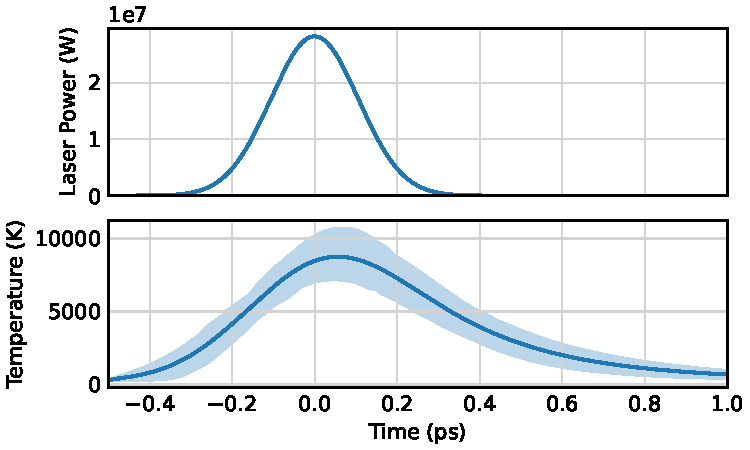
\includegraphics{../analysis/figures/model te.pdf}
    \caption{Calculated electron temperature evolution following femtosecond laser excitation of graphite, showing rapid heating and subsequent cooling through electron-phonon coupling.}
    \label{fig:temperature}
\end{figure}

The excitation of a solid by femtosecond laser pulses can be described using the two-temperature model \cite{roob_thermal_2025,lui_ultrafast_2010}. In this framework, the laser pulse deposits energy into the electron system, raising its temperature \( T_e \), while the lattice remains at its initial temperature \( T_l \). For the short timescales relevant to hot electron dynamics, the lattice temperature can be assumed constant, since thermal diffusion in the lattice occurs much more slowly than electron thermalization.

Under this approximation, the temporal evolution of the electron temperature is governed by

\begin{equation}
C_e(T_e) \frac{\partial T_e}{\partial t} = -G(T_e - T_l) + S(r,t),
\end{equation}

where \( C_e(T_e) \) is the temperature-dependent electronic heat capacity taken from \cite{nihira_temperature_2003}, \( G = \SI{250(50)}{fs}\) \cite{stange_hot_2015} is the electron-phonon coupling constant, and \( S(r,t) \) represents the laser source term. Because the electronic heat capacity is significantly smaller than that of the lattice, the electron temperature can exceed \( T_l \) by several thousand kelvin during the initial femtoseconds after excitation \cite{roob_thermal_2025}. The subsequent cooling proceeds via coupling to optical phonons \cite{lui_ultrafast_2010} and other phonon-mediated relaxation processes \cite{stange_hot_2015}.

Numerical integration of this equation with the utilized laser parameters predicts rapid electronic heating in graphite. \autoref{fig:temperature} shows the resulting electron temperature evolution. The peak electronic temperature exceeds \SI{6000}{K}.

% thermal radiation
The hot electrons emit broadband thermal radiation during their relaxation. Assuming a quasi-equilibrium electron distribution at each moment in time, the instantaneous emission spectrum follows Planck’s law:

\begin{equation}
B(\lambda, T) = \frac{2hc^2}{\lambda^5} \cdot \frac{1}{\exp\left(\frac{hc}{\lambda kT}\right) - 1},
\end{equation}

where \( h \) is Planck's constant, \( c \) is the speed of light, \( k \) is Boltzmann's constant, and \( T \) is the electron temperature. Since the electron temperatures far exceed the lattice temperature during this phase, the electronic thermal emission dominates.

\begin{figure}[b]
    \centering
    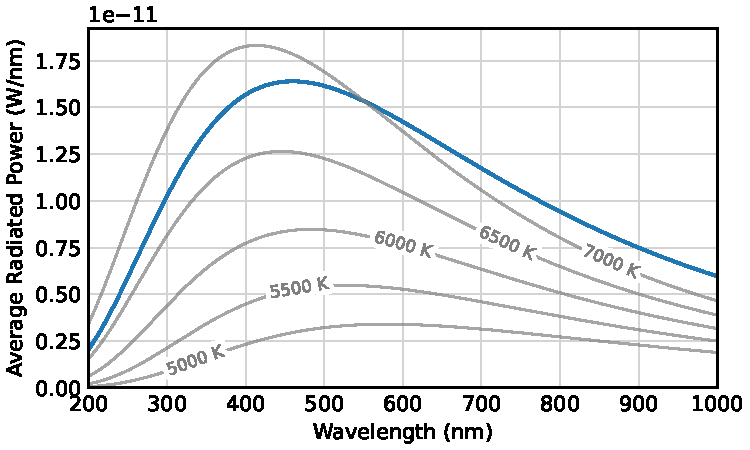
\includegraphics{../analysis/figures/model spectrum.pdf}
    \caption{Calculated thermal radiation spectrum from hot electrons in graphite, obtained by integrating Planck's law over the time-dependent electron temperature. Gray curves show blackbody spectra at constant temperatures, scaled by the effective radiating time.}
    \label{fig:model_spectrum}
\end{figure}

To obtain the total emission spectrum, Planck's law is integrated over the electron cooling curve \( T_e(t) \). \autoref{fig:model_spectrum} shows the result for the same laser parameters as before. The resulting spectrum covers visible and ultraviolet wavelengths. Its smooth shape and theoretical predictability make it a promising candidate for spectral calibration, particularly in the UV where conventional sources are limited.


\section{Experimental Setup}

\begin{figure}
    \centering
    \begin{subfigure}{3.5in}
        \centering
        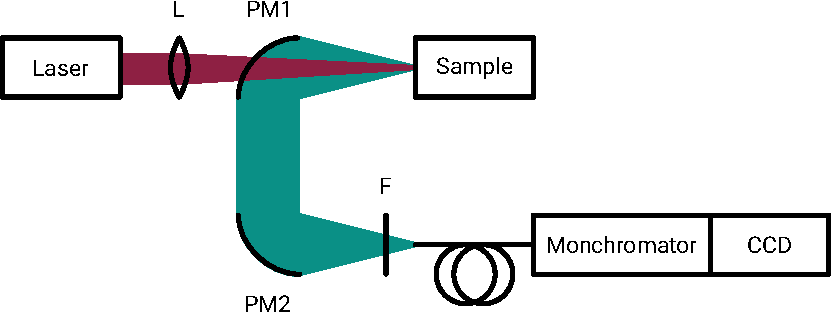
\includegraphics{figures/setup.pdf}
        \caption{Schematic}
    \end{subfigure}
    \hfill
    \begin{subfigure}{2in}
        \centering
        \includegraphics{figures/photo_setup.pdf}
        \caption{Photograph}
    \end{subfigure}
    \caption{Experimental setup used to measure thermal emission from hot electrons. The schematic shows the optical path and key components, while the photograph provides a view of the physical arrangement inside the chamber.}
    \label{fig:setup}
\end{figure}

The experimental setup, originally developed by Leon Roob \cite{roob_thermal_2025}, is shown in \autoref{fig:setup}. It is designed to measure broadband thermal emission from ultrafast-excited hot electrons in graphite using a reflective collection system and fiber-coupled spectrometer.

The excitation source is a Pharos PH1-20 laser (Light Conversion), emitting pulses at \SI{1030}{nm} with a full-width at half-maximum (FWHM) duration of \SI{250}{\femto\second} and a repetition rate of \SI{40}{\kilo\hertz}. The pulse energy was set to \SI{7.5}{\micro\joule}, corresponding to an average power of \SI{300}{\milli\watt}. The beam is stabilized in four axes (position and direction) and expanded to a \SI{5}{\milli\meter} diameter before entering the experiment.

Inside the chamber, the beam is focused onto the sample using a plano-convex lens (L) with a focal length of \SI{200}{\milli\meter}. The resulting spot diameter is approximately \( 4\lambda f / \pi D \approx \SI{50}{\micro\meter} \).

The target material is graphite, mounted on a 3-axis translation stage. Thermal emission from the irradiated spot is collected by a pair of off-axis parabolic mirrors (UV-enhanced aluminum coating). The first mirror (PM1, \SI{50}{\milli\meter} focal length) collimates the emitted light. The second mirror (PM2, \SI{101}{\milli\meter}) focuses it onto a bandpass filter and into a multimode optical fiber with a core diameter of \SI{200}{\micro\meter} (Ocean Optics QP200-2-SR-BX). The magnification factor of this optical system is \( f_{\text{PM2}} / f_{\text{PM1}} = 2 \), resulting in an image spot of approximately \SI{100}{\micro\meter} at the fiber entrance.

The fiber guides the collected light to an Acton SpectraPro 300i monochromator, equipped with a 150\,lines/mm diffraction grating blazed at \SI{500}{\nano\meter}. The dispersed spectrum is detected by an Andor iXon\textsuperscript{EM}+ 897 EMCCD camera operated in vertical binning mode, effectively serving as a 1D line detector.\\
All spectra were corrected by subtracting a dark frame recorded under identical acquisition settings, to remove the detector bias. Wavelength calibration was performed by Leon Roob following the manufacturer's procedure and remained stable throughout the experiment.

To ensure optimal signal and alignment, the lens, sample, and fiber end are mounted on independent precision translation stages. The reflective optics (PM1 and PM2) are fixed relative to the optical axis. Coarse and fine alignment procedures, including the use of a fiber-coupled lamp and real-time spectrometer monitoring, are discussed in the following subsection.

\subsection{Focusing Procedure}
Precise alignment of the sample and optics is essential to maximize coupling efficiency into the spectrometer and ensure reproducible measurements. The focusing process is carried out in several stages, starting with visible light and proceeding to infrared laser optimization.

First, the sample is removed and replaced with a fiber-coupled lamp positioned at the sample location. This visible light source is used to align the optical system by adjusting the lamp position until the output beam appears circular and sharply focused at the spectrometer fiber input. Once a well-defined image is obtained, the spectrometer is connected and positioned to maximize the detected signal. Fine alignment is performed using micrometer screws on the fiber stage, ensuring that the beam spot is centered within the fiber core.

Based on the calculated spot size on the sample of approximately \SI{50}{\micro\meter} and the 2$\times$ magnification of the mirror system, the expected image size at the fiber input is roughly \SI{100}{\micro\meter}, well within the \SI{200}{\micro\meter} core diameter of the multimode fiber. This provides sufficient tolerance for stable alignment, while still requiring careful adjustment for optimal signal.

After completing the optical alignment with the lamp, the sample is reinserted at the same position, and the lamp output is connected to the spectrometer port to illuminate the sample surface. The sample position is then fine-tuned to minimize the visible spot size, indicating the optimal position of the sample.

Finally, the infrared laser is turned on, and an IR detection card is used to locate and focus the beam onto the sample. The reflected laser signal is monitored via the spectrometer, and the laser focus is optimized by adjusting its position to maximize the detected intensity.

This multi-step procedure ensures reliable spatial overlap between the laser excitation and the optical detection axis, enabling consistent measurement of thermal emission from the same region of the sample.


\subsection{Characterization of Noise Sources}

Detecting the weak thermal radiation from hot electrons requires careful optimization of the signal-to-noise ratio (SNR). The dominant noise sources originate from the detector, while laser power fluctuations are assumed negligible.

The EMCCD detector exhibits several characteristic noise mechanisms well-documented by Andor \cite{andor_establishing_nodate,dr_jo_walters_sensitivity_2023} and detailed in \cite{european_machine_vision_association_standard_2010}.

\textbf{Readout noise} represents the fundamental noise floor, arising from charge transfer operations and analog-to-digital conversion. For this high-performance CCD, readout noise measures approximately \SI{1}{e^-} \cite{andor_ixonem_nodate}, consistent with measurements shown in \autoref{fig:dark_noise}. Since this noise applies per readout bin rather than per pixel, hardware vertical binning effectively reduces its impact.

\begin{figure}
    \centering
    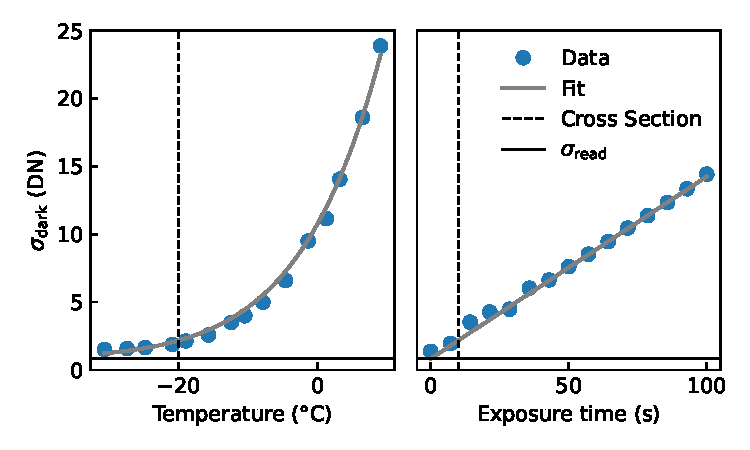
\includegraphics{../analysis/figures/dark_noise.pdf}
    \caption{Dark noise as a function of sensor temperature and exposure time. The fitted curve yields an effective activation energy of $E = \SI{0.597(4)}{eV}$ and constant readout noise of $\sigma_{\text{read}} = \SI{0.81(12)}{e^-}$.}
    \label{fig:dark_noise}
\end{figure}

\textbf{Dark current noise} results from thermal excitation of electrons within the detector semiconductor, following the relationship $N_\text{dark} \propto \exp(-E / kT) \cdot t_\text{exp}$, as demonstrated in \autoref{fig:dark_noise}. Cooling the detector to \SI{-80}{\degreeCelsius} effectively suppresses this contribution, rendering it negligible for typical exposure times.

\textbf{Clock-induced charge noise} scales with electron multiplication gain and signal amplitude. Therefore, sensor gain is deactivated when signal levels significantly exceed readout noise \cite{andor_establishing_nodate}, as in the present configuration.

\textbf{Shot noise} becomes the dominant limitation under these optimized conditions, establishing shot noise-limited operation as shown in \autoref{fig:shotnoise}. The fundamental process begins with incident photons that are converted to photoelectrons with quantum efficiency $\eta$, where the number of generated electrons follows $N_e = \eta \cdot N_{\text{photons}}$. Due to the statistical nature of this conversion process, the variance in the number of photoelectrons equals the mean for Poisson statistics: $\sigma^2 = N_e = \eta \cdot N_{\text{photons}}$ \cite{european_machine_vision_association_standard_2010}.

In practical measurements, the photoelectron signal is amplified by a detector gain $G$, resulting in a measurable output signal $S = G \cdot N_e = G \cdot \eta \cdot N_{\text{photons}}$. The amplification process preserves the Poisson statistics, so the measured noise variance becomes $\sigma^2_{\text{measured}} = G^2 \cdot \eta \cdot N_{\text{photons}}$. This relationship produces the characteristic linear dependence of noise variance on signal intensity observed in \autoref{fig:shotnoise}. \cite{european_machine_vision_association_standard_2010}.

\begin{figure}
    \centering
    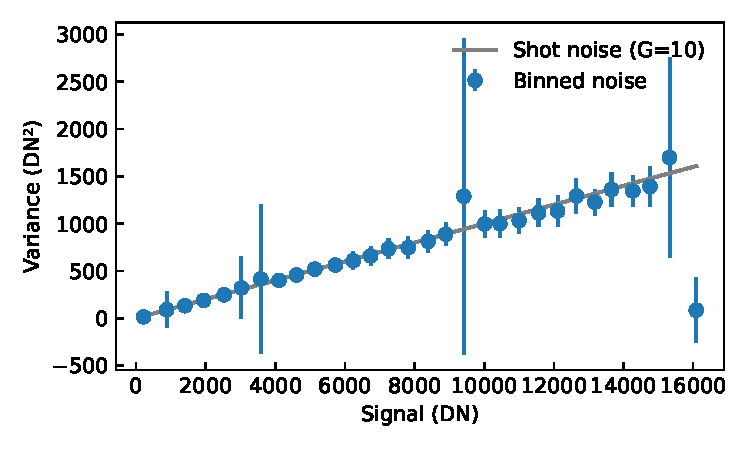
\includegraphics{../analysis/figures/shot noise.pdf}
    \caption{Measured noise versus signal, demonstrating shot noise-limited performance with the characteristic square-root relationship between noise and signal intensity.}
    \label{fig:shotnoise}
\end{figure}

% \section{Detection Efficiency and Calibration Methodology}

% The detection efficiency—defined as the fraction of sample-emitted light reaching the detector—varies with wavelength due to component-specific spectral responses. For physics-based calibration, these individual component responses must be characterized to build the theoretical prediction model.

% The parabolic mirrors and optical fiber exhibit relatively flat spectral responses across the detection range, contributing primarily constant efficiency factors. However, other components introduce wavelength-dependent losses that must be characterized for accurate calibration predictions.

% \begin{figure}
%     \centering
%     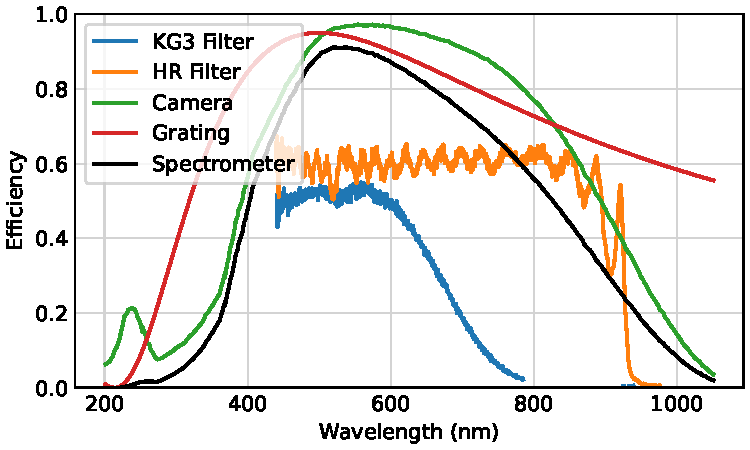
\includegraphics{../analysis/figures/filter.pdf}
%     \caption{Spectral efficiency of optical components in the detection system. Individual component responses combine to determine the overall system efficiency used for comparison with hot electron model predictions in calibration validation.}
%     \label{fig:efficiency}
% \end{figure}

% Spectral filters for laser rejection exhibit distinct transmission characteristics, as shown in \autoref{fig:efficiency}. The SCHOTT KG3 filter, designed for infrared absorption, displays a gradual transmission edge that attenuates expected thermal emission. The HR filter, identified as a dielectric shortpass filter (likely Edmund Optics), shows sharper cutoff behavior, though detailed specifications were unavailable.

% The detector quantum efficiency and grating efficiency curves require more sophisticated characterization. \autoref{fig:efficiency} presents the manufacturer-specified quantum efficiency for the EMCCD camera. Grating efficiency calculations employ the blazed grating model from \cite{barker_ripple_1984}, accounting for wavelength-dependent diffraction characteristics.

% \subsection{Physics-Based Calibration Approach}
% The hot electron calibration methodology combines the two-temperature model predictions with component efficiency characterization to create a complete theoretical framework. Unlike conventional calibration methods that rely on empirically characterized sources, this approach enables prediction of the calibration spectrum from fundamental physical parameters.

% Uncertainties in the theoretical predictions are quantified through Monte Carlo parameter sampling, accounting for variations in laser parameters, material properties, and optical component specifications. This provides built-in uncertainty estimation that is lacking in traditional calibration approaches.

% \subsection{Conventional Calibration Limitations}
% Spectrometer efficiency calibration typically requires reference sources with precisely known spectral characteristics. The standard approach employs calibrated tungsten-halogen lamps with traceable spectral irradiance standards.

% Professional calibration laboratories employ monochromator-based spectral comparator facilities that use silicon photodiode trap detectors previously calibrated against NIST's cryogenic electrical substitution radiometers \cite{houston_achievement_2022,larason_nist_1996}. This approach enables spectral responsivity calibrations with uncertainties below 0.1\% across the visible and near-infrared spectrum.

% \begin{figure}
%     \centering
%     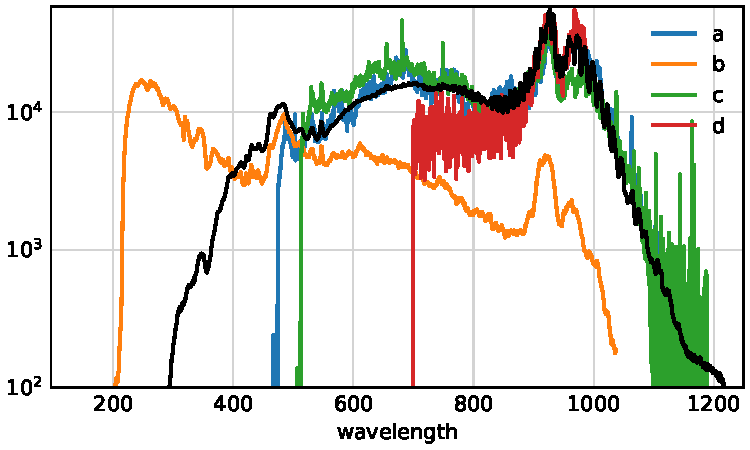
\includegraphics{../analysis/figures/efficiency_different.pdf}
%     \caption{Comparison of identical spectra recorded with different uncalibrated spectrometer systems, demonstrating the calibration discrepancies that arise without proper reference standards.}
%     \label{fig:calibration}
% \end{figure}

% Since no calibrated light source or reference detector with known spectral response was available for this work, an alternative approach using multiple uncalibrated Ocean Optics USB spectrometers was attempted. The broad-spectrum output of a deuterium-halogen lamp (DH-2000-BAL, Ocean Optics) was measured with several different spectrometers to assess consistency. \autoref{fig:calibration} shows the resulting spectra with intensity scaling adjusted for the different instrument sensitivities. The significant disagreement between instruments demonstrates the inadequacy of this approach and underscores the necessity for calibration against traceable reference standards. This comparison illustrates why professional-grade calibration requires the rigorous procedures and metrologically traceable standards maintained by national institutes, rather than relative comparisons between uncalibrated instruments.

\section{Results}

To evaluate the use of hot electron thermal emission as a spectral calibration standard, the measured emission spectrum was compared to model predictions based on the time-dependent electron temperature following femtosecond excitation (see \autoref{fig:model_spectrum}). This comparison provides both a test of the theoretical model and a method to determine the relative spectral efficiency of the detection system.

\begin{figure}
    \centering
    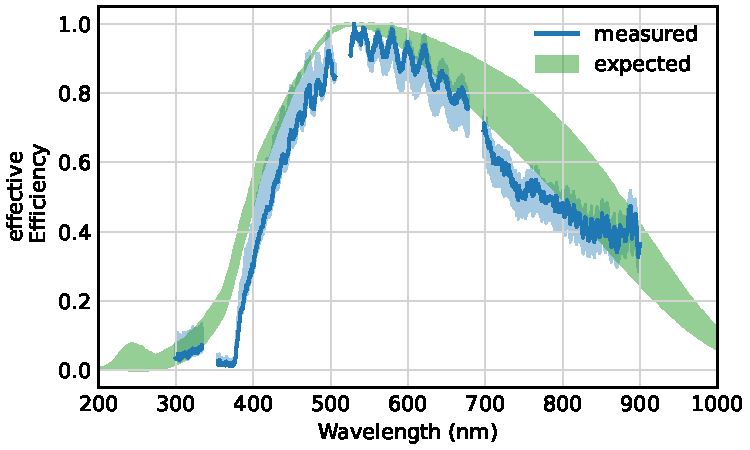
\includegraphics{../analysis/figures/efficiency de.pdf}
    \caption{Model validation and spectrometer efficiency determination. Upper panel: measured thermal emission power density (blue, scaled) versus hot electron model predictions (orange) with uncertainty bands from Monte Carlo parameter sampling. Lower panel: effective spectrometer efficiency derived from model-measurement ratio (blue) compared with expected efficiency from component specifications (orange), demonstrating successful calibration validation.}
    \label{fig:efficiency_comparison}
\end{figure}

\subsection{Model Comparison}

A comparison of the measured thermal emission with the model prediction is presented in the top graph of \autoref{fig:efficiency_comparison}. The simulation is based on the experimental parameters discussed in \autoref{fig:temperature}, with uncertainties captured via Monte Carlo sampling. Parameters such as laser fluence, spot size, reflectivity, and material-specific heat capacity were randomly varied within plausible bounds to generate an ensemble of predicted spectra.

To obtain the measured spectrum in physical units, raw CCD counts were corrected for detector gain and converted to photon flux using the energy–wavelength relationship \(E = hc/\lambda\). A spectral filter was used to suppress harmonic artifacts from the \SI{1030}{nm} excitation laser, isolating the broadband thermal emission. The resulting signal was then scaled to match the model, preserving spectral shape while removing dependence on absolute intensity.

The observed agreement confirms that hot electron thermal emission can be quantitatively modeled from first principles, within the uncertainty bounds of experimental parameters. This validates the core assumption that such emission can serve as a reliable reference for spectral calibration.

\subsection{Efficiency Determination}

The lower graph in \autoref{fig:efficiency_comparison} shows the effective spectral efficiency of the detection system, obtained as the ratio of measured signal to the modeled thermal emission. This curve reflects the combined spectral response of all optical components and the detector, including fiber transmission, mirrors, grating efficiency, and the quantum efficiency of the EMCCD sensor.

For comparison, the manufacturer specifications of the camera and a theoretical model of the grating response (blazed at \SI{500}{nm}) were combined to yield an expected efficiency curve. Both measured and theoretical curves are normalized for shape comparison.

The measured response closely matches the expected shape in the visible range, with peak efficiency around \SI{650}{nm}. Toward shorter wavelengths, however, the measured response drops off more steeply than predicted. This deviation is consistent with known aging effects of antireflection coatings on the EMCCD sensor, which can degrade UV sensitivity over time.

These results highlight two advantages of the proposed method: first, it enables direct detection of spectral response deviations due to component aging or system-specific imperfections; second, it validates that proper optical alignment and modeling allow reliable calibration even in spectral regions where conventional calibration sources are unavailable.

\section{Discussion}

The results demonstrate that thermal emission from hot electrons can serve as a viable reference for the spectral calibration of optical systems, particularly in the UV–VIS range. The comparison between model predictions and measured spectra shows good agreement within the experimental uncertainty, and the derived efficiency curve captures key features expected from the known optical and detector characteristics.

However, several limitations remain. First, the absolute scaling of the model spectrum is subject to uncertainty due to parameters such as laser fluence, spot size, and material reflectivity. While the relative shape of the spectrum is robust and primarily determined by the time-dependent electron temperature, these input parameters introduce amplitude uncertainties that must be accounted for, as done here via Monte Carlo sampling.

Second, the measured efficiency may still include systematic effects not captured by the model, such as fiber coupling losses, imperfect filter transmission, or unaccounted optical reflections. These factors can distort the apparent spectral shape, especially in regions of low signal. Additionally, the assumption of Lambertian emission from the sample may not fully hold in all geometries or for strongly anisotropic surfaces.

Despite these challenges, the method offers a valuable alternative to conventional calibration approaches, particularly when no calibrated UV sources are available. Unlike external lamps, the hot electron emission is generated in situ under actual measurement conditions, automatically accounting for alignment, collection geometry, and spectral filtering. This can reveal performance deviations not captured by factory specifications, such as the observed drop in UV sensitivity due to coating degradation.

Further refinements could include a more precise characterization of the spot size and laser fluence using independent diagnostics, as well as improved modeling of angular emission effects. Additionally, repeated measurements across different days or setups could help identify systematic biases and improve reproducibility.

Overall, this study provides a promising foundation for physics-based calibration using hot electron emission, enabling sensitive and spectrum-resolved efficiency characterization of detection systems in challenging spectral regions.


\section{Conclusion}

This work demonstrates that thermal emission from hot electrons in graphite can serve as a quantitative reference for determining the spectral response of optical detection systems in the UV–VIS range. By comparing measured emission spectra to model predictions based on the two-temperature framework and Planck's law, the relative efficiency of the spectrometer was extracted.

Despite uncertainties in input parameters and potential systematic effects, the agreement between theory and experiment confirms that the emission spectrum can be reliably predicted from first principles. The method thus offers a physics-based alternative to conventional calibration sources, particularly valuable in spectral regions where standard lamps are unavailable or impractical.

Beyond confirming the viability of the approach, the results also reveal performance deviations in the detection system, such as reduced UV sensitivity consistent with known sensor aging effects. This highlights the broader potential of hot-electron emission as an in situ diagnostic tool for characterizing optical systems under real experimental conditions.


\clearpage
\printbibliography

\end{document}